\section{Durchführung}
\label{sec:Durchführung}

Der Versuch wird \autoref{fig:aufbau} entsprechend aufgebaut.

\begin{figure}[H]
    \centering
    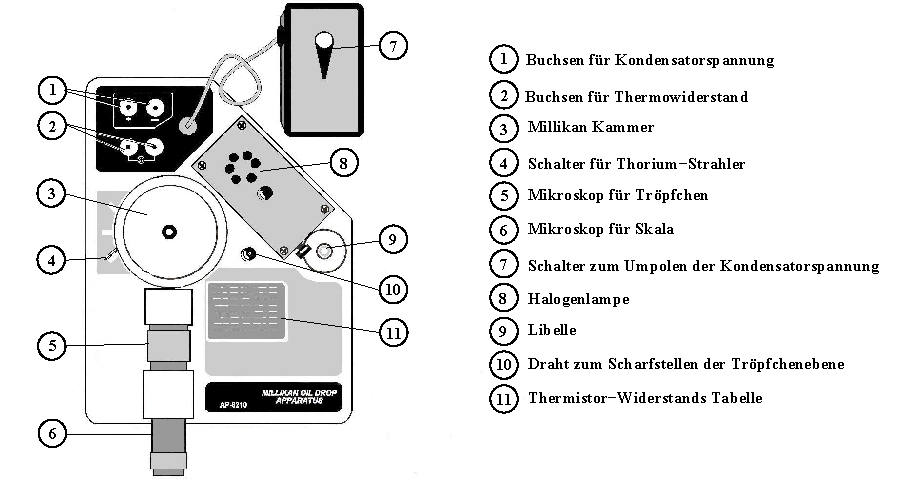
\includegraphics[]{figures/Aufbau.pdf}
    \caption{Beschriftete Abbildung des verwendeten Versuchsaufbaus \cite{v48}.}
    \label{fig:aufbau}
\end{figure}

Da die Probenkristalle hygroskopisch, also Wasser anziehend sind, wird mithilfe der Drehschieber-Vakuumpumpe im Rezipienten, der die Probe enthält, ein Vakuum von etwa $10^{-2} \,\si{\milli\bar}$ aufrechterhalten. 
Die Heizwicklung im Boden des Rezipienten ermöglicht ein Erwärmen der Probe.
Je nach Bedarf kann diese ebenfalls über Kühlfinger abgekühlt werden. Dazu wird das Dewargefäß mit flüssigem Stickstoff gefüllt und so weit nach oben gefahren, dass der Kühlfinger in das Dewar hineintaucht. \\
Die Probentemperatur lässt sich über das im Boden des Rezipienten befindliche Thermoelement ablesen.
Über das angeschlossene Netzgerät kann der Heizstrom so angepasst werden, dass bei der Durchführung eine konstante Heizrate erreicht wird. \\
Eine genauere, schematische Darstellung des Rezipienten findet sich in \autoref{fig:rezipient}.

\begin{figure}[H]
    \centering
    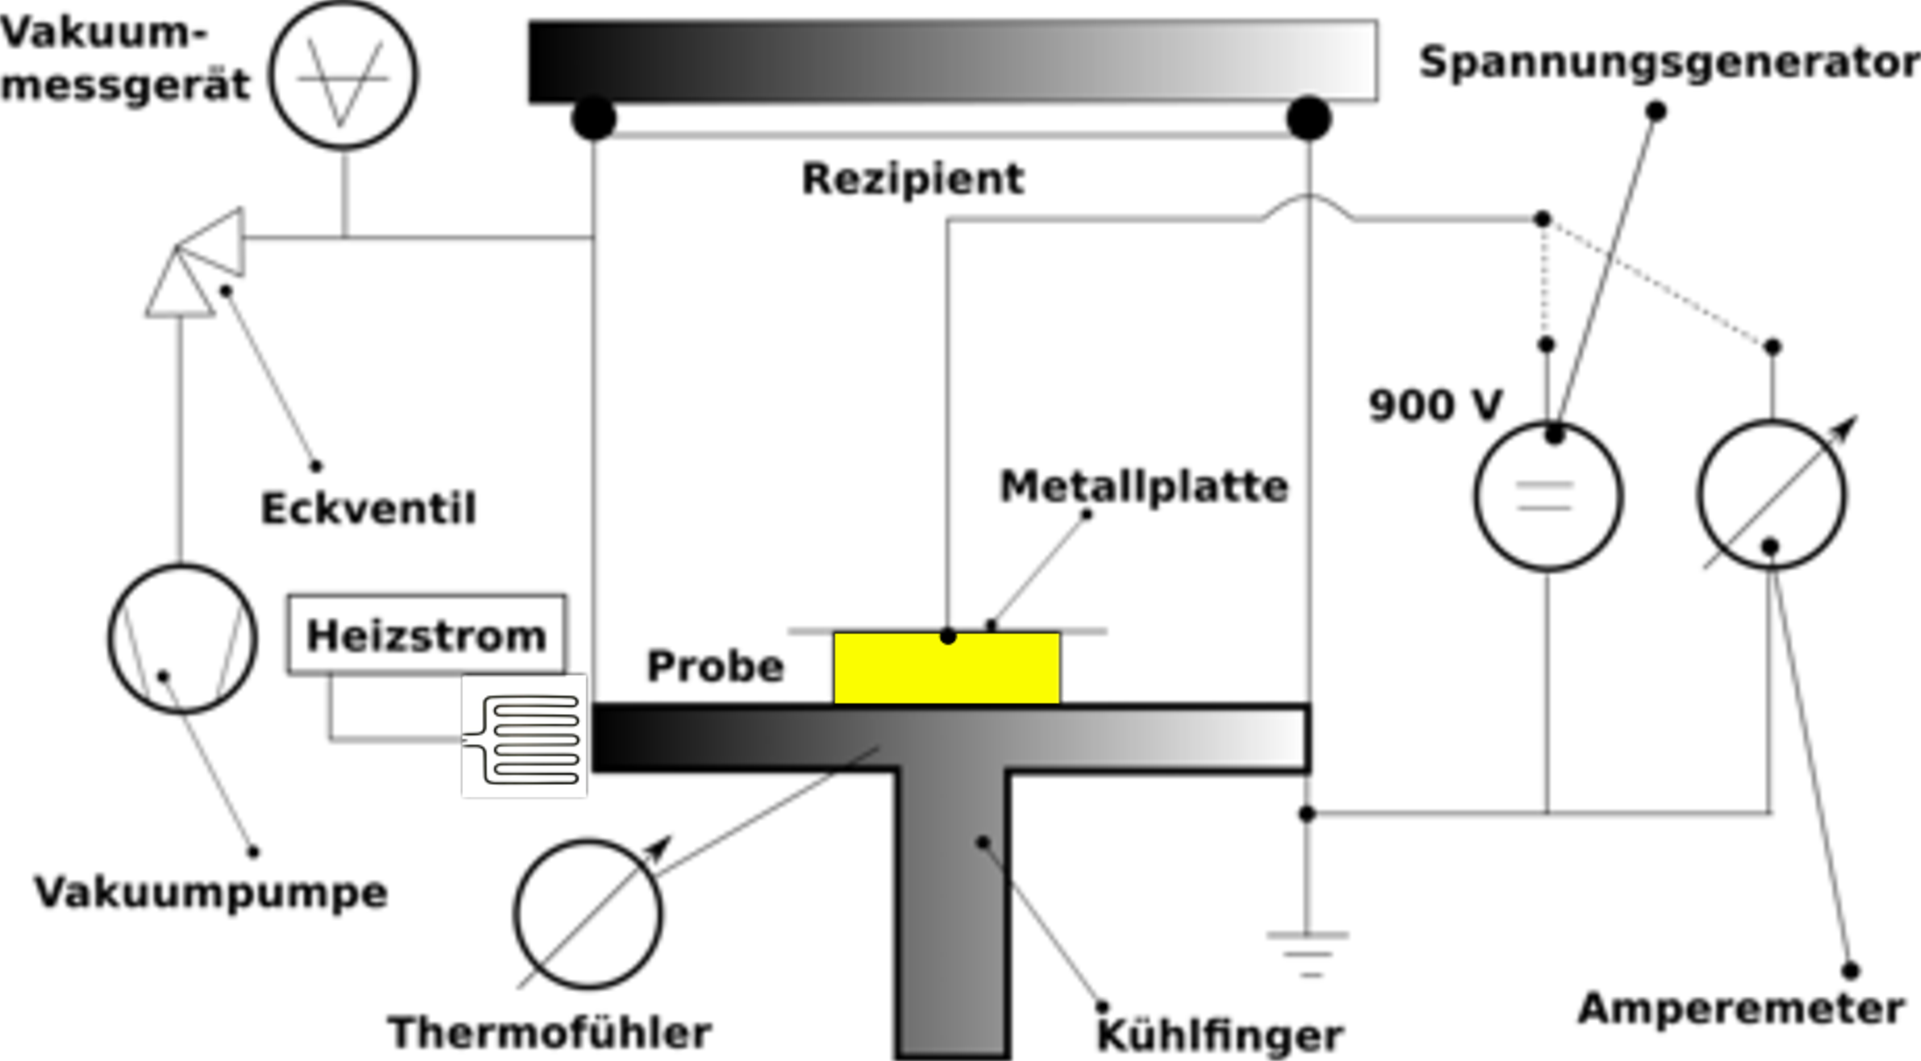
\includegraphics[width=\textwidth]{figures/Rezipient.pdf}
    \caption{Schematische Darstellung des Rezipienten. In gelb ist die Probe dargestellt, die aufliegende Metallplatte ist dieser gegenüber ionisiert und der Rezipient geerdet \cite{v48}.}
    \label{fig:rezipient}
\end{figure}

Vor Beginn der eigentlichen Messreihe wird der Plattenkondensator durch Anlegen eines elektrischen Feldes mit einer Spannung von $950 \,\si{\volt}$ aufgeladen werden.
Dabei ist für die hier verwendete CsI-Probe eine Aufladezeit von $900 \,\si{\second}$ genügend.
Ist der Kondensator aufgeladen, wird die Probe mithilfe von Flüssigstickstoff auf etwa $-50 \,\si{\celsius}$ abgekühlt.
Sobald diese Temperatur erreicht ist, wird das E-Feld abgeschaltet und der Kondensator für $5 \,\si{\minute}$ kurzgeschlossen.
Nach Anschließen des Picoamperemeters sollte ein konstanter Stromwert zwischen $1-2 \,\si{\pico\ampere}$ erreicht werden, bevor mit der Messung begonnen wird.
Dann wird die Probe möglichst gleichmäßig auf etwa $50 \,\si{\celsius}$ erwärmt und der Depolarisierungsstrom in Temperaturabhängigkeit aufgenommen.
Zu Beginn der Messreihe ist die Temperaturdifferenz zur Raumtemperatur hoch genug, um eine genügende Heizrate zu gewährleisten.
Mit steigender Temperatur der Probe wird dann die Heizspannung am Netzteil erhöht.
Dabei wird darauf geachtet, dass die Heizrate einen Wert von $1,5 \, \unit{\frac{\kelvin}{\minute}}$ für die erste und $2,0 \, \unit{\frac{\kelvin}{\minute}}$ für die zweite Messreihe nicht überschreitet. 
Aufgrund der Limitierungen am Netzgerät muss außerdem darauf geachtet, dass keine Heizspannung eingestellt wird, die höher als $110 \,\si{\volt}$ ist. 
